% https://tex.stackexchange.com/q/762992/322482
\documentclass[tikz,border=5pt]{standalone}
\usepackage{fourier}
\usetikzlibrary{bending,patterns.meta,angles,quotes}
\begin{document}
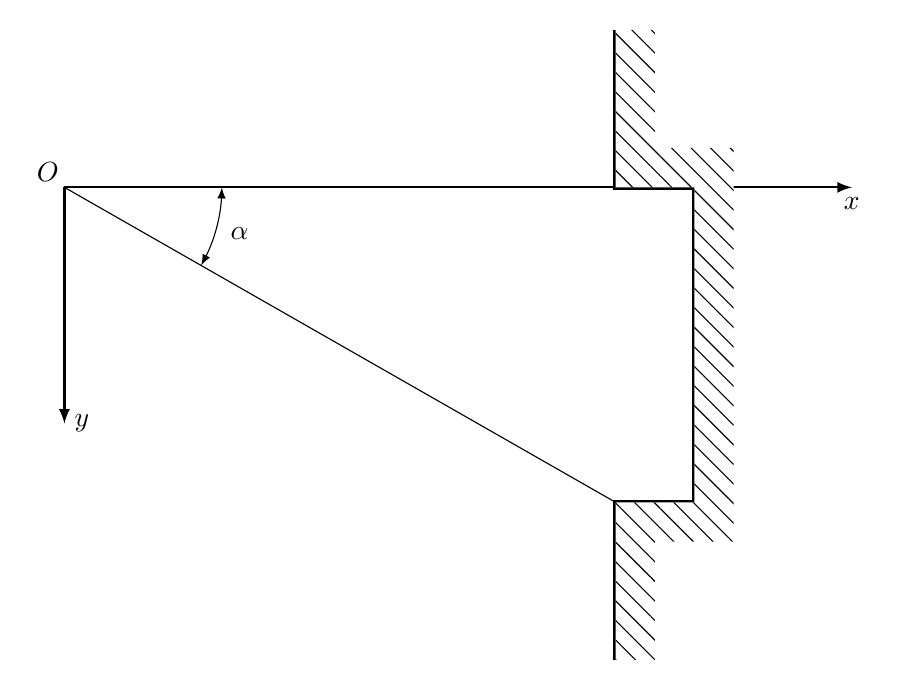
\begin{tikzpicture}[>=latex]
\coordinate (A) at (7,0);
\coordinate (B) at (7,-4);
\newcommand{\mypath}{(7,2) -- (A) -- (8,0) -- (8,-4) -- (B) -- (7,-6)}
  \draw[thick,->] (0,0) -- (10,0) node[below] {$x$};
  \draw[thick,->] (0,0) -- (0,-3) node[right] {$y$};
  \draw[ultra thick] \mypath;
  %%%%%%%%%%%%%%%% path coordinate duplicated
  \fill[pattern={Lines[angle=-45,distance={5pt}]},preaction={fill=white}] \mypath
  -- ++(.5,0) -- ++(0,+1.5) -- ++(1,0) -- ++(0,+5) -- ++(-1,0) -- ++(0,1.5) -- cycle;
  %%%%%%%%%%%%%%%%
  \draw(0,0) node[label={[label distance=-2.5mm]above left:$O$}] (O) {} -- (7,-4) pic[draw,<->,angle radius=2cm,angle eccentricity=1.15,"$\alpha$"] {angle = B--O--A};
\end{tikzpicture}
\end{document}